\documentclass[11pt, oneside]{amsart}
\usepackage{geometry}
\geometry{letterpaper}
\usepackage[francais]{babel}
\usepackage[utf8]{inputenc}
\usepackage{graphicx}
\usepackage{float}
\usepackage{etex,mathtools}
\usepackage{amssymb}
\usepackage{enumitem}
\usepackage{amsmath}
\usepackage{caption}
\usepackage{listings}
\usepackage{array}
\usepackage{hyperref}

%opening
\title{Perceiving physics with computer vision}
\author{Louis Thiry, Marc Sanselme}

\begin{document}

\maketitle

\section*{Introduction}

The goal of this project is to show that a camera can be used as a measuring tool.
To do so, two steps must performed :
\begin{itemize}
  \item Computer vision : determine kinematic informations (positions, angles...) from video.
  \item Learning : use physics equations and learning techniques to deduce physical properties (length, friction coefficient...) from the kinematic informations.
\end{itemize}
We will handle the Computer vision part with convolutionnal neural networks activations.
Concerning the learning technique, we will present a method that is appliable to any physical system whose state $y$ (ex: position, velocity...) is governed by an ordinary differential equation depending on the physical parameters $P$ (mass, length...):
\begin{align*}
  \frac{\partial y}{\partial t} &= F(y, P)\\
\end{align*}
with $F$ differentiable with respect to $P$.
We will illustrate these examples with a pendulum, from which we will learn the length and the friction coefficient.

\section{Determine kinematic informations using CNN activations}

\begin{figure}[H]
\minipage{0.32\textwidth}
  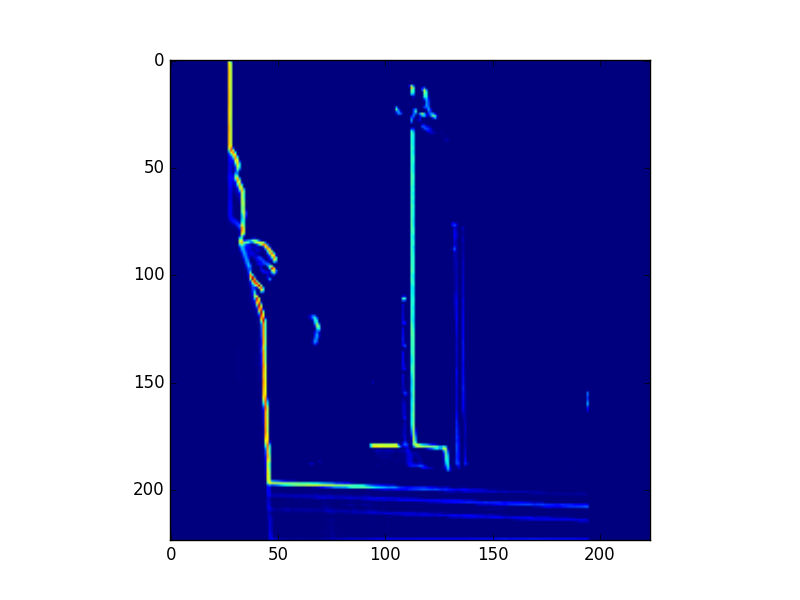
\includegraphics[width=\linewidth]{activation1.png}
\endminipage\hfill
\minipage{0.32\textwidth}
  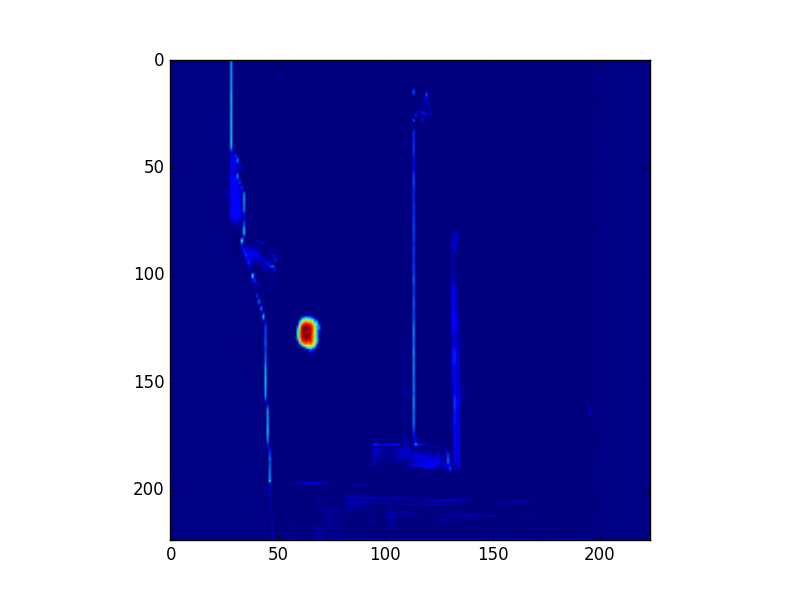
\includegraphics[width=\linewidth]{activation2.png}
\endminipage\hfill
\minipage{0.32\textwidth}%
  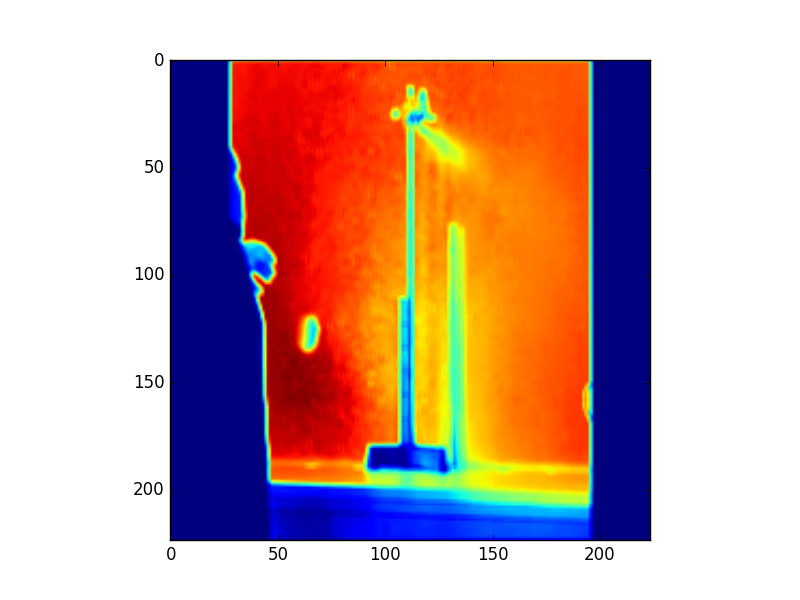
\includegraphics[width=\linewidth]{activation3.png}
\endminipage\hfill
  \caption{Activations at layer 1}
\end{figure}

\begin{figure}[H]
  \captionsetup{labelformat=empty}
  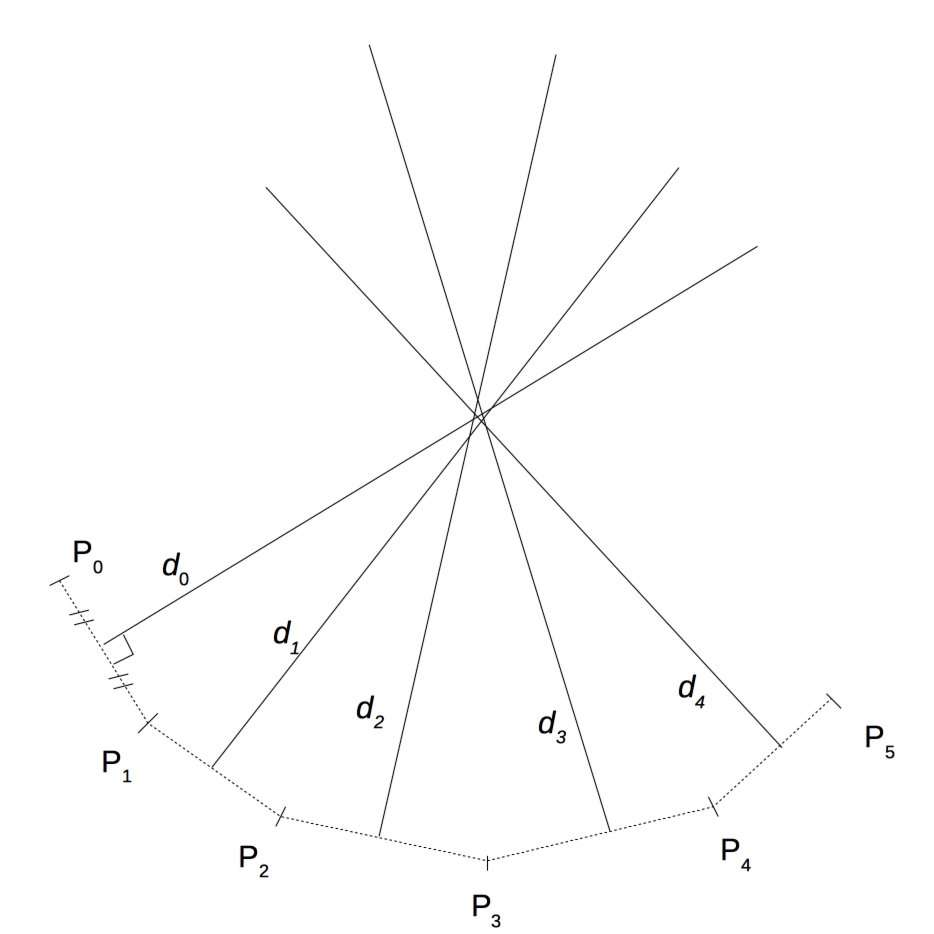
\includegraphics[height=3.5cm]{find_center.png}
  \caption{Find the intersection of lines $d_i$}
\end{figure}

\begin{figure}[H]
  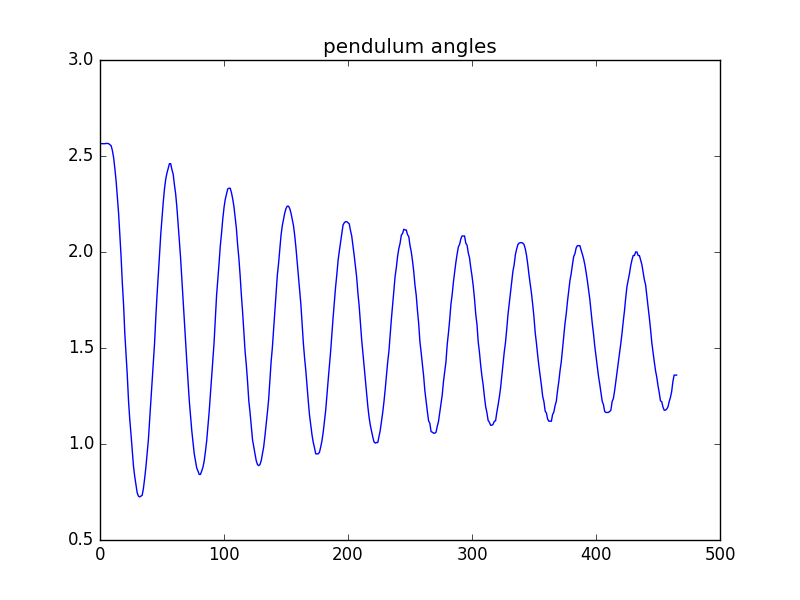
\includegraphics[height=4cm]{pendulum_angles.png}
\end{figure}

\section{Learn physical properties}

We assume that we have a physical system whose state $y$ (ex: position, velocity...) is governed by an ordinary differential equation depending on the physical parameter $P$ (mass, length...):
\begin{align*}
  \frac{\partial y}{\partial t} &= F(y, P)\\
\end{align*}
After the video processing, we have a state sequence $y_n, n=1, \ldots, N$ of observation at time $t = n dt$ where $dt$ is the time step between two frames; and we want to determine the physical parameter $P$ of the system.
For this we use a simple explicit integration of our equation with time step $dt$ to predict $\overline{y}_{t+1}$ knowing $y_t$ : $\overline{y}_{t+1} = y_t + dtF(y_t, P)$ and we want to find the parameter $\hat{P}$ that minimizes the square of the difference between the prediction $\overline{y}_{t+1}$ and the observation $y_{t+1}$ :
\begin{align*}
  \hat{P} &= \underset{P}{\text{argmin }} \sum_{i=1}^{N-1}{\left( y_{t+1} - dtF(y_t, P)\right)^2}\\
\end{align*}
\textbf{Example with a pendulum}\\
The pendulum states is its angle $\theta$ and its angular velocity $\dot{\theta}$.
The parameters are the length $l$ and the friction coefficient $k$.
The equation is :
\begin{align*}
  \frac{d}{dt}\left [ \begin{array}{c} \theta \\ \dot{\theta} \end{array} \right ]
    &=
    \left [ \begin{array}{c} \dot{\theta} \\ -\frac{g}{l}\sin(\theta) - k \dot{\theta} \end{array} \right ]
    \\
\end{align*}
Thus the function $F$ we want to minimize over $k$ and $l$ is :
\begin{align*}
  F(l, k) &= \sum_{i=1}^{N-1}{\left( \dot{\theta}_{t+1} - \dot{\theta_t} + kdt\dot{\theta}_t + \frac{g}{l}\sin(\theta_t) \right)^2}\\
\end{align*}
At the minimum, the partial derivatives over $l$ and $k$ are zero:
\begin{align*}
  \frac{\partial F}{\partial l} &= 0 \implies
    \left( \sum_{t=1}^{N-1}{\sin(\theta_t)(\dot{\theta}_{t+1} - \dot{\theta}_{t}}) \right) +
    k \left( dt \sum_{t=1}^{N-1}{\sin(\theta_t)\dot{\theta}_{t}} \right) +
    \frac{1}{l} \left( gdt \sum_{t=1}^{N-1}{\sin(\theta_t)^2} \right) = 0\\
  \frac{\partial F}{\partial k} &= 0 \implies
    \left( \sum_{t=1}^{N-1}{\dot{\theta_t}(\dot{\theta}_{t+1} - \dot{\theta}_{t}}) \right) +
    k \left( dt \sum_{t=1}^{N-1}{\dot{\theta}_{t}^2} \right) +
    \frac{1}{l} \left( gdt \sum_{t=1}^{N-1}{\sin(\theta_t) \dot{\theta}_t} \right) = 0\\
\end{align*}
which can be easilly solved in close form (done in the code).

For our test video, the learnt values are :
\begin{align*}
  l &= 0.56 \ m\\
  k &= 0.13 \ kg.m^{-1}
\end{align*}


\end{document}
